%!TEX root = ../../super_main.tex
% Skal svare til Ivans: 2.6. Results from representation types and quadrants
% Her skal der tages en masse beslutninger baseret med vision scenarios etc. 
\section{Vision}
\label{sec:vision}
The vision of a solution for this problem is to develop a platform that allows for dynamic collection of data for reality mining. Different area of reality mining require different types of labeled training data. We would like to provide a platform that can gather snapshots which will allow for human activity recognition. The campaigns should be configurable such that it is useful for different purposes, for instance accumulating statistics or to gathering data for training a machine intelligence model. For this reason the platform should allow for configurable collection of snapshots. A customer should be able to to configure what type of informations he wants in the snapshots and how the labels of these should derived, as well as define the demographic group that the campaigns should be available to. The vision for the platform is that people that are in needed of context aware training data, can use our platform instead of developing and distributing their own specialized applications to gather these type of data. The vision for this is to establish a interface for customers where they can specify campaigns, and an interface for participants, in form of a mobile application, that allows for gathering of data for reality mining. An illustration of this can be seen in \figref{fig:system_vision}. Here, customers specify the data the want, through the \emph{uMiner} system. This information is passed along to all mobile devices, which will then know how to mine the reality around the participants. 

\begin{figure}[!htbp]
    \centering
    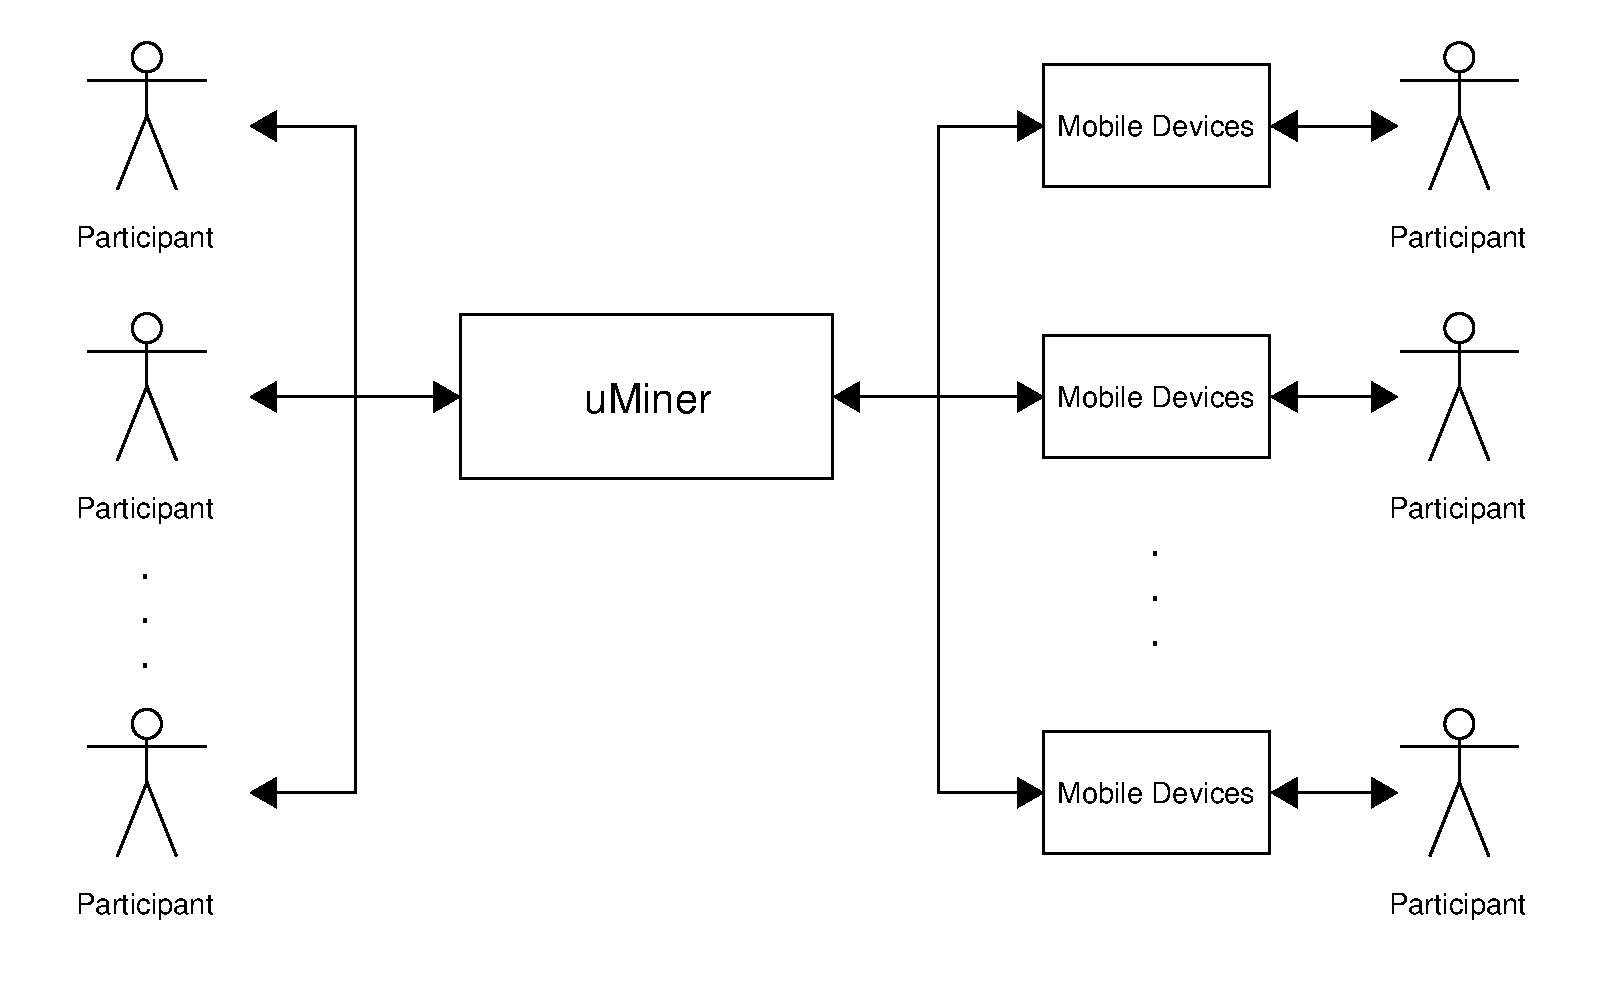
\includegraphics[width=0.8\textwidth]{problem_analysis/vision/system_vision}
    \caption{The system vision.}
    \label{fig:system_vision}
\end{figure}
\FloatBarrier

We imagine that our platform will handle all technical details in regard of gathering the snapshots, and the only task that is left for the customers of this platform is to motivate participants, which they would have to do in any case. Furthermore, this vision requires some collection of data that have potential to violate privacy of the participants of the campaigns, and we will have to consider issues in regards to personal data.

\section{Delimitations}
\label{sec:delimitations}
From the created vision scenarios we learned that the project could include profiles of participants which could allow customers to target specific groups of people with similar demographics. We are certain the ability to target demographics would be valuable to customers but we have however found this would significantly impact the implementability of our solution. We acknowledge the need for customers to have a more select group of people collect data and we have therefore, besides allowing participants to opt-in to campaigns which we will refer to as public campaigns, decided to introduce a concept of private campaigns. A private campaign should work similarly to a public campaign except that the campaign will not be listed publicly in the data gathering application. Access to a private campaign should managed by customers through distribution of an identifier for the campaign. We feel confident that such a simple solution could provide some the same value as including profiles of participants while being easier to implement for first viable version of a solution.

% We could, besides sensors from mobile phones and wearables, also consider including external sensors such as cameras or smart home sensors like movement detectors or temperature sensors in the room. It is however demanding to support many different external sensors in an application, installation of compatible external sensors where the participants reside could entail high installation and maintenance cost and would require a different level of commitment from participants. There has been attempts to alleviate the burden of including many different external sensors in mobile applications by making it easier to interface with them and write drivers but the problem is still considered difficult and costly \parencite{open_data_kit}. We have chosen, at least initially, to not include external sensing as it is deemed too extensive to support collection of such sensors compared to the one of wearables and mobile devices.
